\documentclass[a4paper,11pt]{report}

\usepackage{amsmath,amssymb}
\usepackage{fullpage}
\usepackage{graphicx}

\usepackage{bussproofs}
\usepackage{mathpartir}
\usepackage{prooftrees}
\usepackage{color}

\usepackage{tikz}
\usetikzlibrary{automata,positioning}

\newcommand*\circled[1]{\tikz[baseline=(char.base)]{
            \node[shape=circle,draw,inner sep=2pt] (char) {#1};}}

\makeatletter
\pgfmathdeclarefunction{alpha}{1}{%
  \pgfmathint@{#1}%
  \edef\pgfmathresult{\pgffor@alpha{\pgfmathresult}}%
}

\newcommand*{\until}{U}
\newcommand*{\disj}{\ ,\ }
\newcommand*{\A}{\square}  % Always
\newcommand*{\D}{\diamondsuit} % eventually

\newcommand*{\Pq}{(\top,\bot)}
\newcommand*{\pQ}{(\bot,\top)}
\newcommand*{\PQ}{(\top,\top)}
\newcommand*{\pq}{(\bot,\bot)}


% tikz
\usepackage{tikz}
\usetikzlibrary{snakes}



\author{Sylvain Julmy}
\date{\today}

\setlength{\parindent}{0pt}
\setlength{\parskip}{2.5pt}

\begin{document}

\begin{center}
\Large{
    Automata on Infinite Structure\\
    Fall 2018
  }
  
  \noindent\makebox[\linewidth]{\rule{\linewidth}{0.4pt}}
  Exercice Sheet 6

  \vspace*{1.4cm}

  Author : Sylvain Julmy
  \noindent\makebox[\linewidth]{\rule{\linewidth}{0.4pt}}

  \begin{flushleft}
    Professor : Ultes-Nitsche Ulrich
    
    Assistant : Stammet Christophe
  \end{flushleft}

  \noindent\makebox[\linewidth]{\rule{\textwidth}{1pt}}
\end{center}

\section*{Exercise 1}

\begin{align*}
  \hat{\delta}(\{q_0\},a) &= \{q_0,q_1\} \\
  i_0'((\{q_0\}),a) &= (\{q_0,q_1\}) \\
  i_1'((\{q_0,q_1\})) &= (\{q_0,q_1\})\\
  i_2'((\{q_0,q_1\})) &= (\{q_0\},\{q_1\})\\
  i_3'((\{q_0\},\{q_1\})) &= (\{q_0\},\{q_1\})\\
  \\
  \hat{\delta}(\{q_0\},b) &= \{q_0\} \\
  i_0'((\{q_0\}),a) &= (\{q_0\}) \\
  i_1'((\{q_0\})) &= (\{q_0\})\\
  i_2'((\{q_0\})) &= (\{q_0\},\emptyset)\\
  i_3'((\{q_0\},\emptyset)) &= (\{q_0\})\\
\end{align*}
\begin{align*}
  \hat\delta(\{q_0,q_1\},a) &=  \hat\delta(\{q_0,q_1\},b) = \{q_0,q_1\}\\
  i_0'((\{q_0,q_1\}),a) &= (\{q_0,q_1\},\{q_0\}) \\
  i_1'((\{q_0,q_1\},\{q_0\})) &= (\{q_1\},\{q_0\})\\
  i_2'((\{q_1\},\{q_0\})) &= (\emptyset,\{q_1\},\{q_0\},\emptyset)\\
  i_3'((\emptyset,\{q_1\},\{q_0\},\emptyset)) &= (\{q_1\},\{q_0\})\\
  \\
  i_0'((\{q_0,q_1\}),b) &= (\{q_0\},\{q_1\}) \\
  i_1'((\{q_0\},\{q_1\})) &= (\{q_0\},\{q_1\})\\
  i_2'((\{q_0\},\{q_1\})) &= (\{q_0\},\emptyset,\emptyset,\{q_1\})\\
  i_3'((\{q_0\},\emptyset,\emptyset,\{q_1\})) &= (\{q_0\},\{q_1\})\\
\end{align*}
\begin{align*}
  i_0'((\{q_1\},\{q_0\}),a) &= (\{q_0\},\{q_0,q_1\}) \\
  i_1'((\{q_0\},\{q_0,q_1\})) &= (\emptyset,\{q_0,q_1\}) \\
  i_2'((\emptyset,\{q_0,q_1\})) &= (\emptyset,\emptyset,\{q_0\},\{q_1\}) \\
  i_3'((\emptyset,\emptyset,\{q_0\},\{q_1\})) &= (\{q_0\},\{q_1\})\\
  \\
  i_0'((\{q_1\},\{q_0\}),b) &= (\{q_1\},\{q_0\}) \\
  i_1'((\{q_1\},\{q_0\})) &= (\{q_1\},\{q_0\}) \\
  i_2'((\{q_1\},\{q_0\})) &= (\emptyset,\{q_1\},\{q_0\},\emptyset) \\
  i_3'((\emptyset,\{q_1\},\{q_0\},\emptyset)) &= (\{q_1\},\{q_0\}) \\
\end{align*}

\begin{center}
  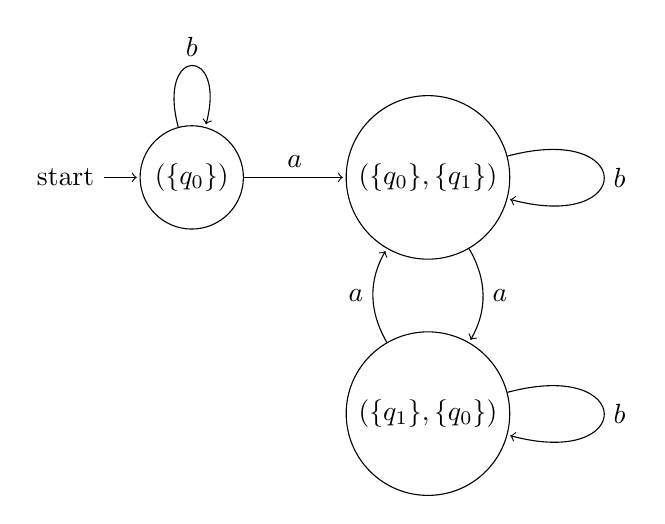
\begin{tikzpicture}[shorten >=1pt,node distance=3cm,on grid,auto]
    \node[state,initial] (q0) {$(\{q_0\})$};
    \node[state] (q0q1) [right = of q0] {$(\{q_0\},\{q_1\})$};
    \node[state] (q1q0) [below = of q0q1] {$(\{q_1\},\{q_0\})$};
    \path[->]
    (q0)
    edge [] node [] {$a$} (q0q1)
    edge [loop above] node [] {$b$} ()
    (q0q1)
    edge [bend left] node [] {$a$} (q1q0)
    edge [loop right] node [] {$b$} ()
    (q1q0)
    edge [bend left] node [] {$a$} (q0q1)
    edge [loop right] node [] {$b$} ()
    ;
  \end{tikzpicture}
\end{center}

\section*{Exercise 2}

\begin{align*}
  i_0'((\{q_0\}),a) &= (\{q_0\}) \\
  i_1'((\{q_0\})) &= (\{q_0\}) \\
  i_2'((\{q_0\})) &=  (\{q_0\},\emptyset)\\
  i_3'((\{q_0\},\emptyset)) &= (\{q_0\}) \\ \\
  i_0'((\{q_0\}),b) &= (\{q_0,q_1\}) \\
  i_1'((\{q_0,q_1\})) &= (\{q_0,q_1\}) \\
  i_2'((\{q_0,q_1\})) &= (\{q_0,q_1\},\emptyset) \\
  i_3'((\{q_0,q_1\},\emptyset)) &= (\{q_0,q_1\}) \\
\end{align*}

\begin{align*}
  i_0'((\{q_0,q_1\}),a) &=  (\{q_0\},\{q_0\})\\
  i_1'((\{q_0\},\{q_0\})) &= (\{q_0\}) \\
  i_2'((\{q_0\})) &=  (\{q_0\},\emptyset)\\
  i_3'((\{q_0\},\emptyset)) &= (\{q_0\}) \\ \\
  i_0'((\{q_0,q_1\}),b) &= () \\
  i_1'() &=  \\
  i_2'() &=  \\
  i_3'() &=  \\
\end{align*}

\begin{align*}
  i_0'(,a) &=  \\
  i_1'() &=  \\
  i_2'() &=  \\
  i_3'() &=  \\ \\
  i_0'(,b) &=  \\
  i_1'() &=  \\
  i_2'() &=  \\
  i_3'() &=  \\
\end{align*}

\begin{center}
  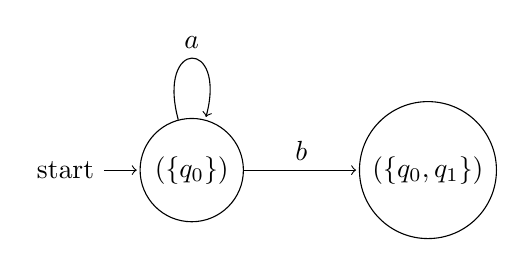
\begin{tikzpicture}[shorten >=1pt,node distance=3cm,on grid,auto]
    \node[state,initial] (q0) {$(\{q_0\})$};
    \node[state] (q0q1) [right = of q0] {$(\{q_0,q_1\})$};
    \path[->]
    (q0)
    edge [loop above] node [] {$a$} ()
    edge [] node [] {$b$} (q0q1)
    (q0q1)
    ;
  \end{tikzpicture}
\end{center}

\end{document}